\subsection{Baseline Definition}
\label{sec:baseline_definition}
As first step we started by trainining the method presented in \cite{mandi2022towards_more_generalizable_one_shot}, using the dataset reported in Section \ref{sec:dataset_description}. In order to valide the trained method we performed 10 rollouts for each variation of each task. For the pick-place task, we performed 160 rollouts and for the nut-assembly task 90 rollouts. We evaluated 3 statistics:
\begin{enumerate*}[label=(\arabic*)]
    \item \textit{Reaching rate}, it evaluates the ratio between the number of times the robot successfully reaches the target objects and the total number of rollouts. Utilizing this metric allows us to assess the system's capacity to identify the target object and guide the robot to reach it;
    \item \textit{Picking rate}, it evaluates the ratio between the number of times the robot pick the target object and the total number of rollouts. This metric takes into account the system's proficiency in executing the picking task, as it necessitates precise control;
    \item \textit{Success rate}, it evaluates the ratio between the number of times the robot complete the given task and the total number of rollouts. This metric considers the system's proficiency in accurately identifying the task's target (e.g., the target bin in pick-place or the target peg in nut-assembly) and generating valid actions to accomplish the task.
\end{enumerate*}
The baseline performance are reported in Table \ref{table:baseline_performance}. With respect to the performance reported in Table \ref{table:mosaic} we observe a relevant performance drop on both pick-place and nut-assembly tasks.
\begin{table}[bth!]
    \centering
    \fontsize{11pt}{11pt}
    \selectfont
    \caption{Baseline performance}
    \label{table:baseline_performance}
    \resizebox{\linewidth}{!}{%
        \begin{tabular}{>{\centering\hspace{0pt}}m{0.298\linewidth}>{\centering\hspace{0pt}}m{0.221\linewidth}>{\centering\hspace{0pt}}m{0.179\linewidth}>{\centering\arraybackslash\hspace{0pt}}m{0.202\linewidth}}
            \hline
            \textbf{Task} & \textbf{Reaching} \par{}\textbf{Rate }\par{}{[}\%] & \textbf{Picking}\par{}\textbf{Rate }\par{}{[}\%] & \textbf{Success}\par{}\textbf{Rate}\par{}{[}\%] \\
            \hline
            Pick-Place    & 66.8                                               & 64.3                                             & 58.7                                            \\
            \hline
            Nut-Assembly  & 40.0                                               & 38.8                                             & 36.6                                            \\
            \hline
        \end{tabular}
    }
\end{table}
\newline Furthermore, for each task, we conducted both quantitative and qualitative analyses of the robot's behavior, focusing on identifying the most pertinent error cases, which are detailed in Table \ref{table:baseline_error_cases}. It is evident from both cases that the most significant error involves the robot successfully completing the task but using the incorrect object, as illustrated in Figure \ref{fig:baseline_pick_place_error}. These findings underscore the system's proficiency in generating valid trajectories but highlight a deficiency in target recognition, as hypothesized in Section \ref{chapter:research_plan}. Consequently, we initiated an assessment of the potential to separate the two tasks inherent in the decision-making process. Potential solutions are discussed in Section \ref{sec:cond_target_obj_detector} and Section \ref{sec:obj_oriented_multi_task_lfd}.
\begin{table}[bth!]
    \caption{Relevant error cases in pick-place task (\ref{table:baseline_pick_place}) and nut-assembly task (\ref{table:baseline_nut_assembly})}
    \label{table:baseline_error_cases}
    \begin{subtable}[h]{0.45\textwidth}
        \centering
        \fontsize{9pt}{9pt}
        \selectfont
        \caption{Relevant error cases in pick-place task}
        \label{table:baseline_pick_place}
        \resizebox{\linewidth}{!}{%
            \begin{tabular}{>{\centering\hspace{0pt}}m{0.475\linewidth}>{\centering\arraybackslash\hspace{0pt}}m{0.406\linewidth}}
                \toprule
                \textbf{Error case}        & \textbf{\#Occurrences} \\
                \hline
                \textbf{Pick wrong object} & \textbf{52}            \\
                \hline
                Place wrong bin            & 6                      \\
                \hline
                Other                      & 8                      \\
                \bottomrule
            \end{tabular}
        }
    \end{subtable}
    \hfill
    \begin{subtable}[h]{0.45\textwidth}
        \centering
        \fontsize{9pt}{9pt}
        \selectfont
        \caption{Relevant error cases in nut-assembly task}
        \label{table:baseline_nut_assembly}
        \resizebox{\linewidth}{!}{%
            \begin{tabular}{>{\centering\hspace{0pt}}m{0.475\linewidth}>{\centering\arraybackslash\hspace{0pt}}m{0.406\linewidth}}
                \toprule
                \textbf{Error case}        & \textbf{\#Occurrences} \\
                \hline
                \textbf{Pick wrong object} & \textbf{45}            \\
                \hline
                Fail to pick               & 9                      \\
                \hline
                Other                      & 2                      \\
                \bottomrule
            \end{tabular}
        }
    \end{subtable}

\end{table}
\begin{figure}[bth!]
    \centering
    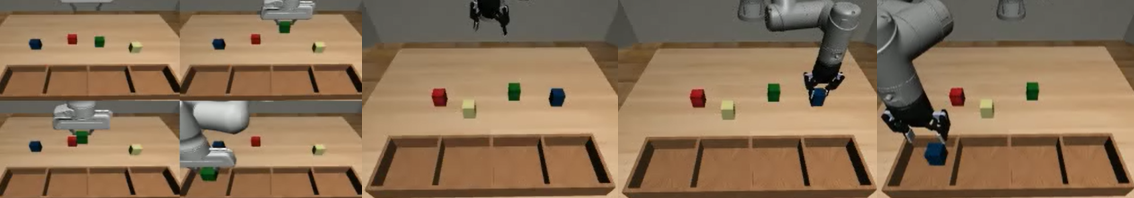
\includegraphics[width=0.6\textwidth]{Figures/images/baseline_pick_place_error/pick_place_trj.png}
    \caption{Example of error where the robot complete the task but with a wrong object}
    \label{fig:baseline_pick_place_error}
\end{figure}

